\section{Numerical model and benchmark scenarios}
\label{sec:model}

\subsection{Train--track--bridge interaction model}
\label{sec:ttbi}

The vehicle responses are generated with a two-dimensional, vertically coupled
train--track--bridge interaction (TTBI) model implemented in MATLAB and derived
from the TTB-2D/VEqMon2D framework of Cantero~\cite{cantero_ttb2d,
cantero2022veqmon}, the framework used by Fernandes et
al.~\cite{fernandes2025early}. The model (Fig.~\ref{fig:model}) couples (i) an
Euler--Bernoulli bridge deck on vertical support springs, with rotational
springs at the end bearings; (ii) a layered track with rail, pads, sleepers,
ballast, and sub-ballast~\cite{zhai2004track}; and (iii) a train of five
identical planar vehicles, each with bounce and pitch degrees of freedom for
the carbody and the two bogies and four wheelsets that follow the rail. The
vehicle properties follow the intercity-train calibration of O'Brien et
al.~\cite{obrien2018vehicle}. The wheel--rail interaction is linear and
bilateral, and the coupled equations of motion are integrated with the
average-acceleration Newmark method ($\gamma=1/2$, $\beta=1/4$) using a time
step of 1~ms. The generator is a modified version of the published TTB-2D code,
distributed under the GPL-3.0 license; the damage models and data-generation
scripts are additions of the present authors. Table~\ref{tab:parameters} lists
the main parameters.

\begin{figure}[htbp]
\centering
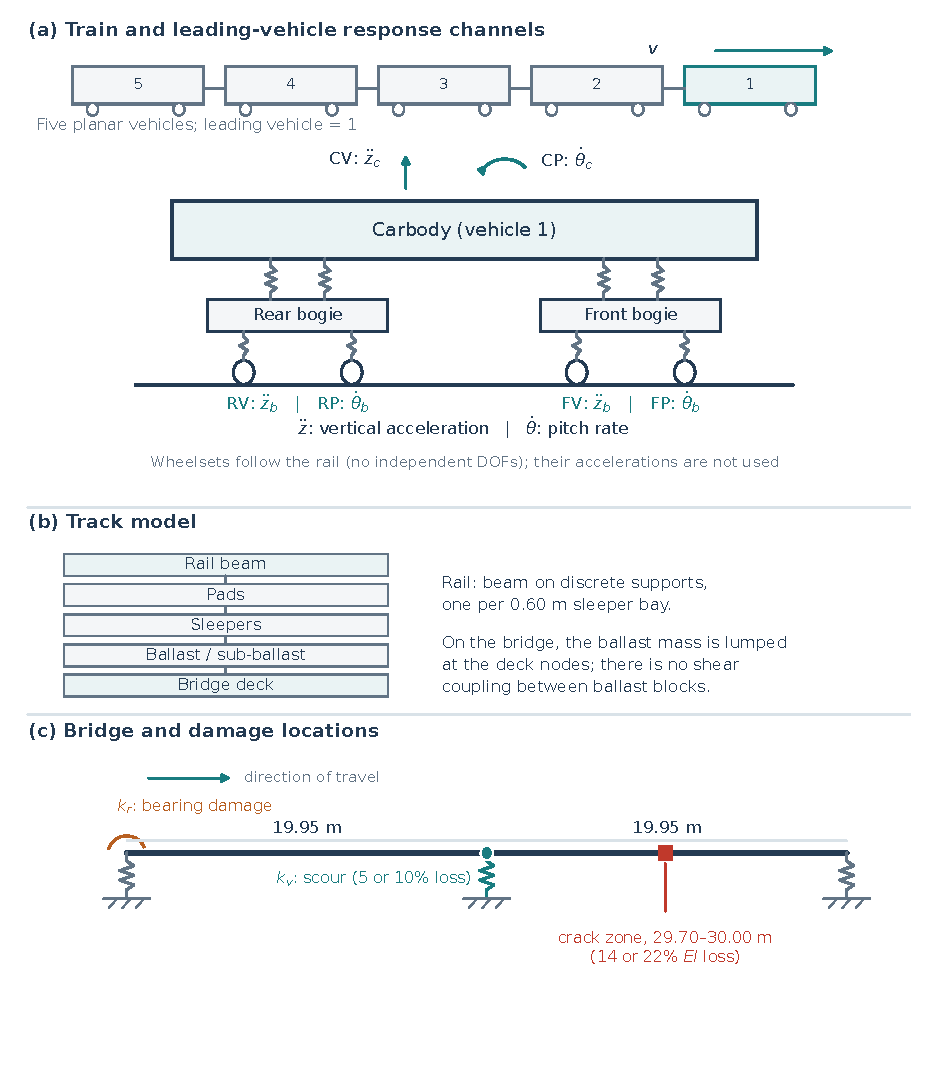
\includegraphics[width=0.92\textwidth]{ttbi_model.pdf}
\caption{Planar train--track--bridge interaction model (not to scale): (a)
five-vehicle train and the six responses of the leading vehicle considered in
this study; (b) track model; (c) two-span bridge with the locations of the
scour, bearing, and crack damage.}
\label{fig:model}
\end{figure}

The track parameters follow Zhai et al.~\cite{zhai2004track} with the planar
conventions of the code. The rail bending stiffness and mass correspond to two
rails, and the sleeper mass is complete, whereas the pad, ballast, and
sub-ballast properties are the values that Zhai et al.\ report per rail seat,
placed on a sleeper spacing of 0.60~m. On the bridge, the ballast mass of each
sleeper is lumped at the corresponding deck node, and the shear coupling
between adjacent ballast blocks is omitted. The bridge has 3\% Rayleigh damping,
and the rail 0.1\%, with coefficients computed from the first two vertical
bending modes of each bridge configuration; a change of support or flexural
stiffness therefore also changes the damping matrices. These conventions are the
same in all scenarios. Because the contact is bilateral, every passage was
checked for tensile wheel--rail forces; none occurred, and no loss of contact
was recorded in any of the 2,000 passages.

\begin{table}[htbp]
\centering
\caption{Nominal parameters of the train--track--bridge interaction model. Track
values follow the planar conventions described in Section~\ref{sec:ttbi}.}
\label{tab:parameters}
\footnotesize
\setlength{\tabcolsep}{4pt}
\resizebox{\textwidth}{!}{%
\begin{tabular}{llll}
\toprule
Subsystem & Parameter & Value & Units \\
\midrule
\multirow{8}{*}{Bridge}
 & spans & $2\times19.95$ & m \\
 & Young's modulus $E$ at 15\,$^{\circ}$C & $35\times10^{9}$ & N/m$^2$ \\
 & second moment of area $I$ & 0.33 & m$^4$ \\
 & mass per unit length & 9,600 & kg/m \\
 & Rayleigh damping ratio, first two modes & 3 & \% \\
 & healthy vertical stiffness of the central support $k_v$ & $3.44\times10^{8}$ & N/m \\
 & healthy first vertical frequency & $\approx4.1$ & Hz \\
 & deck element length & 0.15 & m \\
\midrule
\multirow{8}{*}{Track}
 & rail bending stiffness $EI$ (two rails) & $1.325\times10^{7}$ & N$\cdot$m$^2$ \\
 & rail mass (two rails) / Rayleigh damping ratio & 121.28 / 0.1 & kg/m, \% \\
 & pad stiffness / damping & $6.5\times10^{7}$ / $7.5\times10^{4}$ & N/m, N$\cdot$s/m \\
 & sleeper spacing / mass & 0.600 / 251 & m, kg \\
 & ballast mass / stiffness / damping & 531.4 / $1.3775\times10^{8}$ / $5.88\times10^{4}$ & kg, N/m, N$\cdot$s/m \\
 & sub-ballast stiffness / damping & $7.75\times10^{7}$ / $3.115\times10^{4}$ & N/m, N$\cdot$s/m \\
 & rail element length & 0.30 & m \\
 & rail extension beyond the model ends & 6 & m \\
\midrule
\multirow{7}{*}{Vehicle ($\times5$)}
 & carbody mass / pitch inertia & 36,852 / 560,342 & kg, kg$\cdot$m$^2$ \\
 & bogie mass / pitch inertia & 3,910 / 10,024 & kg, kg$\cdot$m$^2$ \\
 & wheelset mass & 1,407 & kg \\
 & primary suspension stiffness / damping per axle & $5.558\times10^{6}$ / $5.88\times10^{4}$ & N/m, N$\cdot$s/m \\
 & secondary suspension stiffness / damping per bogie & $2.0\times10^{6}$ / $1.2\times10^{5}$ & N/m, N$\cdot$s/m \\
 & bogie-centre spacing / axle spacing & 16 / 2.3 & m \\
 & vehicle length / wheel radius & 22 / 0.46 & m \\
\midrule
Solver & Newmark-$\beta$ ($\gamma=1/2$, $\beta=1/4$); time step & $10^{-3}$ & s \\
\bottomrule
\end{tabular}%
}
\end{table}

\subsection{Bridge and damage scenarios}
\label{sec:scenarios}

The bridge is the two-span railway viaduct of the source study. The source text
describes two 20~m spans, whereas its finite-element grid of 133 elements of
0.30~m corresponds to a 39.9~m deck with two 19.95~m spans; the latter geometry
is reproduced here. The deck is discretized into 266 elements of 0.15~m. This
uniform refinement keeps every node of the source grid and places the central
support, which lies inside an element of the source grid, on a node. Both end
bearings of the healthy bridge are free to rotate~\cite{fernandes2025early}.

Table~\ref{tab:f25_scenarios} lists the ten scenarios. Scour is represented by a
5\% or 10\% reduction of the vertical stiffness $k_v$ of the central support.
Bearing damage is represented by a rotational stiffness of $10^{9}$~N\,m/rad at
the entrance bearing, a value adopted by the source as the lowest level of
bearing damage detectable by drive-by monitoring. The source models a crack
with the tapered flexural-rigidity law of Sinha et
al.~\cite{sinha2002simplified} at the mid-span of the second span and reports
that crack-depth ratios of 0.10 and 0.05 correspond to $EI$ reductions of
approximately 22\% and 14\% for a 0.30~m element. Here those reductions are
applied uniformly over the same 0.30~m zone, $29.70\le x\le30.00$~m, which
consists of two refined elements. The crack-depth ratios are kept as class
labels; they are not depths calibrated for the uniform model.

\begin{table}[htbp]
\centering
\caption{Damage scenarios of the benchmark~\cite{fernandes2025early}. The crack
label is the source crack-depth ratio; the simulated damage is the listed
uniform $EI$ reduction. Bearing damage is the rotational restraint of the
entrance bearing.}
\label{tab:f25_scenarios}
\small
\begin{tabular}{lrrrc}
\toprule
Scenario & Crack label (\%) & $EI$ reduction (\%) & Scour, $k_v$ reduction (\%) & Bearing damage \\
\midrule
Healthy & 0 & 0 & 0 & -- \\
DC2 & 10 & 22 & 0 & -- \\
DC3 & 0 & 0 & 5 & -- \\
DC4 & 0 & 0 & 0 & yes \\
DC5 & 0 & 0 & 10 & yes \\
DC6 & 10 & 22 & 10 & -- \\
DC7 & 10 & 22 & 0 & yes \\
DC8 & 10 & 22 & 10 & yes \\
DC9 & 10 & 22 & 5 & yes \\
DC10 & 5 & 14 & 5 & yes \\
\bottomrule
\end{tabular}
\end{table}

\subsection{Operational variability and simulated measurements}
\label{sec:eov}

Each scenario is simulated for 200 passages, giving 2,000 passages. For each
scenario a Latin hypercube~\cite{mckay1979comparison} of 17 variables is drawn:
the train speed (70--90~km/h), the temperature (3--33~$^{\circ}$C), and, for each
of the five vehicles, the carbody mass (33,000--40,000~kg) and the primary and
secondary suspension stiffnesses (2,640--2,920 and 942--1,042~kN/m per side,
doubled in the planar model). These are the ranges of the source
study~\cite{fernandes2025early}. Temperature modifies the deck modulus as
$E(T)=E_{15}\,[1-0.003\,(T-15)]$. The rail irregularity is the stored FRA
class-4 profile realization used by Fernandes et
al.~\cite{fernandes2024driveby, fernandes2025early}; it is the same for every
passage and scenario.

Following the source, the responses of the leading vehicle are monitored while
its axles cross the bridge, approximately from the entry of the first axle to
the exit of the last one, and are resampled at 100 samples/m. The source reports
a 58.3~m window of 5,830 samples. Its window convention, which uses a 40~m
bridge term, yields 5,831 inclusive samples on the present grid, and the last
sample is discarded. The resulting window is nine samples (0.09~m) longer than
a window computed with the exact 39.9~m deck length.

\subsection{Response channels}
\label{sec:response_channels}

Six responses of the leading vehicle are considered (Table~\ref{tab:channels}
and Fig.~\ref{fig:model}a): the vertical accelerations and the pitch rates of
the carbody and of the two bogies. The carbody responses are filtered by the
primary and secondary suspensions, whereas the bogie responses are filtered by
the primary suspension only. The source study used the vertical accelerations
of the carbody (CV) and of the front bogie (FV). Wheelset accelerations are not
used: in the planar model the wheelsets follow the rail, so their accelerations
are kinematic quantities rather than independent responses.

\begin{table}[htbp]
\centering
\caption{Responses of the leading vehicle considered in this study.}
\label{tab:channels}
\small
\begin{tabular}{lll}
\toprule
Code & Response & Used in the source study \\
\midrule
CV & carbody vertical acceleration & yes \\
FV & front-bogie vertical acceleration & yes \\
RV & rear-bogie vertical acceleration & no \\
CP & carbody pitch rate & no \\
FP & front-bogie pitch rate & no \\
RP & rear-bogie pitch rate & no \\
\bottomrule
\end{tabular}
\end{table}
